\section{IP mapping}
L'ultimo problema che viene descritto è anche l'ultimo problema di cui io ed il
prof. Anisetti ci siamo accorti, in ordine cronologico; ed è stato anche il problema
più difficile da risolvere, e che, potenzialmente, avrebbe potuto far fallire
tutto il lavoro precedentemente fatto, ma procediamo con ordine.

\subsection{Il problema}
Si è detto in precedenza che si è scelta infine una configurazione \textit{Multi Local
Server}, con i server OpenVPN installati in MoonCloud e raggiungibili mediante IP
pubblici da i client presenti nella rete target. Per ragioni di costi, si vuole
limitare il numero di VM in MoonCloud con OpenVPN in esecuzione, e quindi poter
dedicare un singolo server a servire più reti target contemporaneamente. OpenVPN
consente di isolare i singoli client connessi ad un server, infatti di default
tali client possono comunicare solo con il server, e non con altri client (a meno
che si utilizzi la direttiva ``\texttt{client-to-client}'', e, come si è visto,
tale direttiva non viene utilizzata).\\
Per poter quindi realizzare in maniera corretta una topologia del genere è
\textit{fondamentale che ogni rete target abbia un spazio di indirizzamento diverso}\ldots
Tuttavia qui sorge il problema: ciascuna LAN target è ragionevolmente dotata
di uno o più pool di indirizzi privati, i quali sono limitati. L'RFC \cite{rfc-private-addr}
stabilisce che i seguenti spazi di indirizzi siano riservati per l'utilizzo esclusivo
in una rete privata e che non siano instradabili su Internet:
\begin{itemize}
  \item classe A (subnet mask a 8 byte) \texttt{10.0.0.0} -- \texttt{10.255.255.255}
  \item classe B (subnet mask a 16 byte) \texttt{172.16.0.0} -- \texttt{172.31.255.255}
  \item classe C (subnet mask a 24 byte) \texttt{192.168.0.0} -- \texttt{192.168.255.255}
\end{itemize}
Spesso accade poi che tali indirizzi siano utilizzati con una subnet mask non
\textit{canonica}, ad esempio si può utilizzare \texttt{10.1.1.0/24}, rimane
comunque il fatto che i detti prefissi sono tipicamente quelli che si trovano
in una qualsiasi LAN.\\
Nell'estate del 2014 ho lavorato per tre mesi in una azienda che si occupava di
gestire la parte IT di altre aziende, e, sebbene non mi vanti di avere una grande
esperienza in merito, ho potuto constatare come nei fatti solo \textit{alcuni}
degli indirizzi sopra citati siano utilizzati, ad esempio ho visto usati
spesso indirizzi nel range \texttt{10.1.1.0/24} -- \texttt{10.10.10.0/24} e
\texttt{192.168.1.0/24} -- \texttt{192.168.100.0/24}.\\
E' quindi chiaro come la probabilità che due reti target di due clienti diversi
abbiano lo stesso spazio di indirizzamente sia piuttosto alta. Diventa
quindi un grosso problema poter collegare più
reti target ad uno stesso VPN server, proprio perché avranno uno stesso indirizzo IP
di rete.\\
Una prima soluzione potrebbe essere quella di destinare ad ogni server un certo
numero di reti target predefinite, ad esempio al server \texttt{OpenVPN10-20}
si assegnano le reti nello spazio \texttt{10.0.0.0/24} -- \texttt{10.20.20.0/24},
e così via fino ad esaurire lo spazio di indirizzi privati. Ogni volta che
si collega una nuova rete target, essa viene assegnata al server VPN competente
sulla base del suo indirizzo di rete\ldots Chiaramente questa soluzione non è
possibile, si possono individuare almeno tre problematiche:
\begin{itemize}
  \item cosa fare nel caso due reti target diverse abbiano lo stesso indirizzo IP?
  \item Cosa fare nel caso in cui cliente sia dotato di più reti, che per competenza
  spetterebbero a diversi server OpenVPN? Non è possibile collegare uno stesso client
  a due server contemporaneamente.
  \item Molti server infine resterebbero poco utilizzati, perché sebbene, ad esempio,
  siano responsabili per venti target, ne hanno assegnate solo un paio. Viceversa,
  altri sarebbero utilizzati fino al proprio limite.
\end{itemize}
Un'altra soluzione potrebbe essere quella di allocare un server OpenVPN
\textit{per ogni} cliente, sia che esso abbia una oppure $n$ reti che debbano essere
analizzate da MoonCloud. Lato MoonCloud si creano quindi tante reti isolate tra loro
costituite da un server OpenVPN e da un \textit{Docker host}, ciascuna competente
per un singolo cliente. Questa configurazione risolve effettivamente il problema di
conflitto tra reti target diverse, poiché si assume che un singolo cliente, nel caso
in cui sia composto da più di una rete, abbia configurato le proprie reti con indirizzi
di rete \textit{diversi}.\\
Perché non adottare quindi questa soluzione? La risposta è semplice, perché avrebbe
fatto lievitare i costi di MoonCloud alle stelle, richiedendo di allocare un altissimo
numero di VM per OpenVPN server, e più clienti MoonCloud acquisisce, più questi
costi aumenterebbero!\\
Ecco quindi il problema a cui ho dovuto trovare una soluzione: \textit{come gestire
la conflittualità tra gli indirizzi IP delle reti target senza dover allocare un
server OpenVPN per ogni cliente?}
Prima di analizzare la risposta a tale quesito, si meglio cosa succederebbe in caso in cui
vi siano dei pacchetti generati da dei \textit{probe} destinati ad una delle due reti target,
e che vi
sia un conflitto di indirizzamenti. Si ipotizza di lavorare nella seguente
configurazione:
\begin{itemize}
  \item rete target 1: \texttt{192.168.100.0/24} (cliente $A$)
  \item rete target 2: \texttt{192.168.100.0/24} cliente ($B$)
  \item rete MoonCloud: \texttt{192.168.200.0/24}
  \item indirizzo IP interno VPN server: \texttt{192.168.200.20}
  \item indirizzo IP pubblico VPN server: \texttt{100.4.78.5}
  \item indirizzo IP del \textit{Docker host} per client $A$: \texttt{192.168.200.2}
  \item indirizzo IP del \textit{Docker host} per client $B$: \texttt{192.168.200.3}
  \item indirizzo IP VPN client $A$: \texttt{192.168.100.50}
  \item indirizzo IP VPN client $B$: \texttt{192.168.100.150}
  \item subnet VPN: \texttt{10.7.0.0/24}
  \item indirizzo IP scheda di rete virtuale VPN server: \texttt{10.7.0.1}
  \item indirizzo IP scheda di rete virtuale VPN client $A$: \texttt{10.7.0.2}
  \item indirizzo IP scheda di rete virtuale VPN client $B$: \texttt{10.7.0.3}
  \item \texttt{CommonName} del VPN client $A$: \texttt{clientA}
  \item \texttt{CommonName} del VPN client $B$: \texttt{clientB}
\end{itemize}
Si supponga infine che si adottano le soluzioni discusse precedentemente, tra cui
l'uso del \textit{NAT al contrario}, ed il \textit{NAT lato server}. Le direttive
``\texttt{iroute}'' dei file di configurazione relativi ai due client contengono
entrambi l'indicazione della rete \texttt{192.168.100.0 255.255.255.0}.
Ciò che si descrive di seguito è \textit{ipotetico}, poiché non è nemmeno detto che
OpenVPN accetti due \texttt{iroute} di due client diversi con lo stesso contenuto,
supponendo che ciò sia possibile, accadrebbe la situazione che ora si dettaglia.
\begin{enumerate}
  \item Un \textit{probe} per client $A$ genera un pacchetto, la sorgente di tale pacchetto è
  \texttt{192.168.200.2}, la destinazione \texttt{192.168.100.254}; si supponga che
  tale pacchetto sia una richiesta HTTP a tale indirizzo (e che quindi sia un TCP \texttt{SYN}).
  \item Il sistema operativo del \textit{Docker host A} consulta la propria routing table
  ed instrada il pacchetto verso \texttt{192.168.200.20}
  \item contemporaneamente, un altro \textit{probe} per client $B$ genera un pacchetto,
  la sorgente di tale pacchetto è
  \texttt{192.168.200.3}, e la sfortuna vuole che la destinazione sia
  \texttt{192.168.100.254}, e che in questo caso si tratti di un pacchetto  di inizio
  di una connessione SSH.
  \item Il sistema operativo del \textit{Docker host B} consulta la propria routing table
  ed instrada il pacchetto verso \texttt{192.168.200.20}
  \item il sistema operativo del VPN server riceve il pacchetto da \texttt{192.168.200.2},
  consulta la
  routing table e trova l'entry \texttt{192.168.100.0/24 via 10.7.0.1}, quindi inoltra
  alla scheda di rete virtuale di OpenVPN
  \item il sistema operativo del VPN server riceve il pacchetto da \texttt{192.168.200.3},
  consulta la
  routing table e trova l'entry \texttt{192.168.100.0/24 via 10.7.0.1}, quindi inoltra
  alla scheda di rete virtuale di OpenVPN
  \item OpenVPN riceve i due pacchetti,
  essi hanno entrambi come destinazione \texttt{192.168.100.254}
  \item OpenVPN consulta la propria routing table e trova che sia client $A$ sia client $B$
  sono responsabili per tali pacchetti, per cui si supponga (non è dato sapere come OpenVPN
  si comporti davvero in questo caso\footnote{Non è dato sapere come OpenVPN si comporterebbe
  davvero in un caso come questo, né lo si è verificato in pratica perché ci si è
  piuttosto concentrati sulla soluzione di tale probelma.}) che entrambi i due pacchetti
  siano inviato ad entrambi i due client.
  \item Entrambi i due pacchetti sono ricevuti da \texttt{clientA}, il quale provvede
  a scriverli sulla propria scheda di rete virtuale
  \item i pacchetti sono quindi ricevuti dal sistema operativo ed inviati a
  \texttt{192.168.100.254} nella rete $A$
  \item parallelamente, i due pacchett sono ricevuti da \texttt{clientB} ed inviati a
  \texttt{192.168.10.254} nella rete $B$.
  \item A questo punto si possono verificare diverse combinazioni più o meno
  sfortunate, qua se ne elenca solo una, ma abbastanza esemplificativa:
  \begin{itemize}
    \item \texttt{192.168.100.254} $A$ li riceve e li elabora, si supponga che per una sfortunata
    coincidenza su tale host sia installato sia un server HTTP (a cui era destinato il
    pacchetto proveniente da \texttt{192.168.200.2}) sia un server SSH: entrambi
    producono delle risposte ``valide'' per i due pacchetti.
    \item \texttt{192.168.100.254} $B$ riceve anch'esso i due pacchetti e li elabora, si ricorda
    che a tale host era destinato solo un pacchetto per il server SSH, e che non vi
    sia alcun server HTTP. Per tale motivo, la risposta al pacchetto SSH è una
    risposta ``valida'', mentre invece la risposta alla richiesta HTTP, si supponga
    sulla porta 80, produce un \texttt{connection reset by peer}\footnote{Il protocollo TCP
    prescrive che quando si invii un \texttt{SYN} verso una porta chiusa si risponda
    con un \texttt{RST}.}.
  \end{itemize}
  \item i due host nelle due reti inoltrano quindi le risposte ai due client VPN, i quali
  applicano il NAT ed inviano al server OpenVPN
  \item per ragioni non note, i pacchetti di risposta provenienti dalla rete del cliente $B$
  arrivano prima al server, OpenVPN provvede quindi a scriverli sulla scheda di rete
  virtuale
  \item il sistema operativo li riceve ed riapplica il NAT, ed ora iniziano i veri problemi:
  si supponga che \texttt{iptables} riesca ad applicare il NAT ad entrambi i pacchetti
  (si ricorda che quello contenente l'\texttt{RST} di risposta ad un web server non esistente
  è una risposta che non dovrebbe esistere)
  \item il pacchetto di risposta al TCP \texttt{SYN} per l'instaurazione di una connessione
  in vista della richiesta HTTP viene inviato al \textit{Docker host} \texttt{192.168.200.2},
  il cui \textit{probe} vedrà quindi un risultato diverso da quello reale (il pacchetto
  di risposta dalla rete $A$ deve ancora arrivare)
  \item il pacchetto di risposta all'inizio della connessione SSH (sarà un
  \texttt{SYN/ACK}) viene ricevuto dal \textit{Docker host} \texttt{192.168.200.3} e quindi
  inviato al \textit{probe}, in questo caso il \textit{probe} vedrà il risultato reale.
  \item Ora il server OpenVPN riceve i due pacchetti provenienti dalla rete $A$, che sono
  quindi scritti sulla scheda di rete virtuale e ricevuti dal sistema operativo
  \item \texttt{iptables} dovrebbe riapplicare NAT come descritto tre punti prima, che cosa
  succede? Si riesce ad applicare il NAT? Anche ammesso che si riesca, le risposte
  arriverebbero duplicate, ammesso che non vengano scartate o che si verifiche qualche
  altra anomalia.
\end{enumerate}
E' quindi chiaro che, qualsiasi cosa succeda, i \textit{probe} raramente riceveranno
le risposte legittime, e durante il percorso possono verificarsi molti incovenienti che
facciano sì che tale risposte addirittura non raggiungano \textit{mai} i probe. Si
ribadisce che lo scenario descritto è \textit{ipotetico}, non è nemmeno detto che OpenVPN
accetti la situazione di conflitto presente nei file di configurazione client-specific.

\subsection{La soluzione}
Mentre questo problema emergeva con il prof. Anisetti, la prima soluzione che entrambi
abbiamo abbozzato è stata quella in cui MoonCloud \textit{rimappi} ogni rete target
su una nuova rete, stabilita da MoonCloud e garantita essere univoca.
``\textit{Rimappare}'' una rete significa trovare una nuovo NET ID per tale rete, e
\textit{spostare} gli indirizzi IP originali nel nuovo NET ID. Lato MoonCloud, i
\textit{probe} conoscono gli indirizzi IP modificati (garantiti univoci), ed il rimappaggio
verso quelli originali viene effettuato sul device VPN client.\\
Entrambi concordi che questa fosse la soluzione corretta, si trattava ora di capire
come potessa il client rimappare gli indirizzi IP, tenendo presente che tale
rimappaggio deve essere perfettamente aderente a quello stabilito da MoonCloud.
Prima di proseguire, si chiarisce meglio la terminologia che da qui in poi sarà utilizzata:
\begin{itemize}
  \item ``\textit{rete originale OTN (Original Target Network)}'': l'indirizzo IP di rete della rete target così come
  è in realtà
  \item ``\textit{IP originale OTI (Original Target IP)}'': l'indirizzo IP di un
  host nella rete target così
  come è in realtà
  \item ``\textit{rete mappata MTN (Mapped Target Network)}'': il nuovo NET ID
  assegnato ad una rete target
  \item ``\textit{IP mappato MTI (Mapped Target IP)}'': l'indirizzo IP appartenente alla \textit{rete
  mappata} a cui corrisponde un indirizzo IP originale
  \item ``\textit{rete rimappata RTN (Remapped Target Network)}'':  l'indirizzo
  IP di rete della rete target così
  come è in realtà, ovvero uguale alla \textit{rete originale}
  \item ``\textit{IP rimappato RTI (Remapped Target IP)}'': corrisponde all'\textit{IP originale}.
  \item ``\textit{mappare una rete}'': assegnare alla \textit{rete originale} una
  \textit{rete mappata}
  \item ``\textit{mappare un indirizzo IP}'': assegnare un \textit{IP mappato}
  ad un \textit{IP originale}
  \item ``\textit{rimappare una rete}'': procedimento inverso del
  ``\textit{mappare una rete}''
  \item ``\textit{rimappare un indirizzo IP}'': procedimento inverso del
  ``\textit{mappare un indirizzo IP}''
  % \item ``\textit{SMTN (Set of Mappped Target Networks)}'': l'insieme di reti mappate
\end{itemize}
Il motivo per cui esistono due sinonimi sarà presto chiaro. Si definiscono quindi
le seguenti funzioni \textit{deterministiche} (con $S$ corrispondente ad un certo
server OpenVPN):
\begin{itemize}
  \item $map\_network: OTN, S \rightarrow MTN$, una funzione cha data una
  $OTN$ ritorna una $MTN$, garantita univoca per ogni server
  \item $map\_address: OTI, OTN, MTN, S \rightarrow MTI$,
  una funzione che dato in input:
  \begin{itemize}
    \item $OTI \mid OTI \in OTN$: un indirizzo IP originale appartenente alla
    rete originale
    \item $OTN$: la rete originale
    \item $MTN \mid map\_network(OTN)=MTN$: la rete mappata della rete originale
    \item $S$: il server OpenVPN a cui $OTN$ è assegnata
  \end{itemize}
  ritorni $MTI$: un indirizzo $\in MTN$ corrispondente a $OTI$.
  \item $remap\_network: MTN, S \rightarrow OTN$, una funzione che data una rete
  mappata ritorna la corrispondente rete originale assegnata ad un certo server,
  con $OTN=RTN$.
  \item $remap\_address: MTI, MTN, OTN, S \rightarrow OTI$, una funzione che dato
  in input:
  \begin{itemize}
    \item $MTI \in MTN$: indirizzo IP mappato
    \item $MTN \mid map\_network(OTN)=MTN$: la rete $OTN$ mappata
    \item $OTN$: la rete originale
    \item $S$  il server OpenVPN a cui $OTN$ è assegnata
  \end{itemize}
  ritorna $OTI$: un indirizzo $\in OTN$ corrispondente a $MTN$, e $RTI=OTI$
\end{itemize}
Per queste funzioni valgono le seguenti uguaglianze:
\begin{itemize}
  \item $remap\_network(map\_netowrk(OTN, S), S)=map\_network(OTN, S)^{-1}$
  \item
  $remap\_address(map\_address(OTN, OTI, MTN, S), MTN, OTN, S)=\\
    map\_address(OTN, OTI, MTN, S)^{-1}$
\end{itemize}
In altre parole, ogni funzione è l'inverso dell'altra.\\
\textit{Come effettuare il mappaggio?} Per rispondere a questa domanda, si vede ora
un nuovo flusso che include questa nuova funzionalità.
Si supponga di avere la seguente configurazione:
\begin{itemize}
  \item rete target $OTN$: \texttt{192.168.100.0/24}
  \item rete mappata: $map\_network(OTN, S)=$\texttt{192.168.1.0./24}
  \item rete MoonCloud: \texttt{192.168.200.0/24}
  \item indirizzo IP interno VPN server $S$: \texttt{192.168.200.20}
  \item indirizzo IP pubblico VPN server: \texttt{100.4.78.5}
  \item indirizzo IP del \textit{Docker host}: \texttt{192.168.200.2}
  \item indirizzo IP VPN client ($OTI \in OTN$): \texttt{192.168.100.50}
  \item subnet VPN: \texttt{10.7.0.0/24}
  \item indirizzo IP scheda di rete virtuale VPN server: \texttt{10.7.0.1}
  \item indirizzo IP scheda di rete virtuale VPN client: \texttt{10.7.0.2}
  \item \texttt{CommonName} del VPN client: \texttt{client1}
  \item target da analizzare ($OTI \in OTN$): \texttt{192.168.1.254}
  \item target mappato: $MTI \in MTN=map\_address(\texttt{192.168.100.254},\\
  \texttt{192.168.100.0/24},
  \texttt{192.168.1.0/24})=\texttt{192.168.1.254}$
\end{itemize}
Le reti mappate sostituiscono le reti originali nella configurazione delle rotte lato
MoonCloud. Quindi si mostra un estratto dei file \texttt{client-up.sh} e
\texttt{client-down.sh}, come si può vedere, la rotte aggiunte e rimosse sono
quelle mappate.
\begin{minted}[breaklines]{bash}
#! /bin/bash

# /etc/openvpn/server/cs/client-up.sh


if [ "$common_name" == "client1" ]; then
  ip route add 192.168.1.0/24 via 10.7.0.1
  iptables -t nat -A POSTROUTING -d 192.168.1.0/24 -j MASQUERADE
fi
\end{minted}
\begin{minted}[breaklines]{bash}
#! /bin/bash

# /etc/openvpn/server/cs/client-down.sh


if [ "$common_name" == "client1" ]; then
  ip route del 192.168.1.0/24 via 10.7.0.1
  iptables -t nat -D POSTROUTING -d 192.168.1.0/24 -j MASQUERADE
fi
\end{minted}
Allo stesso modo, il file \texttt{client1} che contiene le direttive client-specific
avrà il seguente contenuto:
\begin{minted}{bash}
iroute 192.168.1.0 255.255.255.0
\end{minted}
Infine, per applicare la soluzione di \textit{NAT al contrario}, sul device client
sarà eseguito il comando \texttt{iptables}:
\begin{minted}[breaklines]{bash}
iptables -t nat -A POSTROUTING -d 192.168.100.0/24 -s 10.7.0.0/24 -j MASQUERADE
\end{minted}
Si noti che in questo comando la rete di destinazione è la \textit{rete originale}.\\
 I passi eseguiti sono quindi i seguenti:
\begin{enumerate}
  \item un cliente registra una nuova rete: \texttt{192.168.100.0/24}
  \item MoonCloud sceglie a quale server $S$ assegnare tale rete,
  in questo caso è il VPN server all'indirizzo IP interno \texttt{192.168.200.20}
  \item MoonCloud mappa la rete in input $MTN=map\_network(\texttt{192.168.100.0/24}, S)$,
  ed $MTN=\texttt{192.168.1.0/24}$
  \item si crea un nuovo device client, proriamente configurato
  \item il device client viene collegato alla rete target e si connette al server OpenVPN
  \item si alloca un nuovo \textit{Docker host}, nell'esempio in questione è \texttt{192.168.200.2}
  \item il cliente configura una nuova analisi, specificando come target: \texttt{192.168.100.254}
  \item il target di tale analisi passato ai \textit{probe} è il risultato dell'applicazione
  di $map\_address(\texttt{192.168.100.254}, \texttt{192.168.100.0/24}, \texttt{192.168.1.0/24})$,
  ovvero \texttt{192.168.1.254} (detto $MTI$)
  \item il \textit{probe} genera un pacchetto destinato a \texttt{192.168.1.254}, cioè $MTI$
  \item il sistema operativo del \textit{Docker host} ha configurato una rotta del tipo:
  \texttt{192.168.1.0/24 via 192.168.200.20}, quindi il pacchetto viene inviato al server VPN
  \item il sistema operativo del server $S$ riceve il pacchetto, a sua volta ha configurato
  la rotta seguente: \texttt{192.168.1.0/24 via 10.7.0.1}; tale rotta è stata configurata
  tramite il file di script \texttt{client-up.sh}.
  \item a questo punto il pacchetto passa nello stato di \texttt{POSTROUTING}, e come
  si applica la regola di NAT descritta nel file sopra, quindi l'IP sorgente del
  pacchetto in questione è ora \texttt{10.7.0.1}
  \item il pacchetto viene inviato all'interfaccia
  virtuale di OpenVPN, e da esso ricevuto
  \item OpenVPN consulta la propria routing table interna, in conseguenza di ciò quindi
  invia il pacchetto a \texttt{Client1} lungo la connessione TCP con esso
  \item il pacchetto viene ricevuto dal device client, l'indirizzo IP di destinazione è
  quello mappato, cioè \texttt{192.168.1.254}
  \item il pacchetto viene scritto sull'interfaccia virtuale e ricevuto dal kernel
  del sistema operativo
  \item in un modo che poi verrà descritto, il sistema operativo di \texttt{Client100}
  applica la seguente funzione
  per ottenere $OTI=RTI$ cioè l'indirizzo IP effettivo del target: $OTI=remap\_address(
  \texttt{192.168.1.254}, \texttt{192.168.1.0/24},\\ \texttt{192.168.100.254})$, il
  risultato è \texttt{192.168.100.254}, il quale ovviamente corrisponde all'indirizzo IP
  specificato dal cliente come target dell'analisi.
  \item Si modifica l'indirizzo IP destinazione del pacchetto, inserendo come destinazione
  $OTI$, cioè \texttt{192.168.100.254}
  \item a questo punto il pacchetto è in stato di \texttt{POSTROUTING} e si applica il
  \textit{NAT al contrario}, l'indirizzo IP sorgente è ora \texttt{192.168.100.50}
  (cioè l'IP del device client)
  \item il pacchetto viene quindi inviato a \texttt{192.168.100.254}
  \item \texttt{192.168.100.254} riceve il pacchetto, lo elabora, invia una risposta
  con destinazione \texttt{192.168.100.50}
  \item il pacchetto viene ricevuto da \texttt{192.168.100.50} (\texttt{Client100}),
  come prima cosa
  si riapplica l'inverso di \textit{NAT al contrario}, modificando l'indirizzo IP
  destinazione in \texttt{10.7.0.1} (l'indirizzo IP sorgente del pacchetto di richiesta
  inviato dal server OpenVPN)
  \item il sistema operativo di \texttt{Client1} ora provvede a modificare tale
  pacchetto, andando a specificare che l'indirizzo IP sorgente non è più
  \texttt{192.168.100.254} (IP originale -- $OTI$), ma \texttt{192.168.1.254}
  (IP mappato -- $MTI$). Per farlo, applica:
  $source=map\_address(\texttt{192.168.100.254}, \texttt{192.168.100.0/24},\\
  \texttt{192.168.1.0/24})$
  ; a questo il pacchetto è conforme a quello inviato da OpenVPN server dopo il
  \textit{NAT lato server}, poiché l'indirizzo IP sorgente è quello mappato, cioè quello
  che MoonCloud conosce.
  \item il sistema operativo quindi inoltra il pacchetto alla scheda di rete virtuale
  OpenVPN, il quale lo riceve e lo invia al server
  \item il server OpenVPN $S$ riceve il pacchetto, lo decifra, lo scrive sulla scheda di rete
  virtuale
  \item il sistema operativo del server $S$ lo riceve, a questo punto si riapplica
  il \textit{NAT lato server}, l'indirizzo IP destinazione passa da \texttt{10.7.0.1}
  a \texttt{192.168.200.2}: a questo punto preciso \textit{il pacchetto è esattamente
  la risposta precisa alla richiesta generata dal Docker host}.
  \item Il pacchetto viene quindi inviato al \textit{Docker host} e quindi al \textit{probe}.
\end{enumerate}
Poiché questa descrizione è abbastanza lunga, è possibile trovarne una più schematica
nella prossima sezione: \textit{configurazione finale}.\\
Detto questo, non resta che spiegare \textit{come} eseguire le funzioni di mappaggio
e rimappaggio.


Lato server, $map\_network$ è una funzione eseguita dal microservizio da me scritto
e che sarà dettagliato nel prossimo capitolo. Per ora basti sapere che nel momento
in cui avviene l'\textit{enrollment} di un nuovo cliente, le sue reti sono mappate
su nuove reti in modo che siano univoche.\\
Ogni volta che si specifica un target per l'analisi, il cliente inserisce l'indirizzo IP
\textit{vero} ($OTI$), quindi si contatta il mio microservizio per ottenerne
la sua versione mappata ($MTI$): tale indirizzo $MTI$ è l'IP target dei \textit{probe}
che fanno analisi.\\
All'interno di MoonCloud, ogni vi sono varie reti locali che comprendono il VPN server,
responsabile per un certo numero di clienti, ed un certo numero di \textit{Docker host}
i quali effettivamente fanno l'analisi tramite tale server. Ogni rete è isolata
dalle altre, pertanto è possibile che due server VPN abbiano due reti target mappate
uguali, ma questo non crea conflitto perché i due server sono isolati tra loro.
Allo stesso modo, un server è ovviamente in grado di gestire più clienti
contamporaneamente, poiché l'univocità delle reti mappate è garantita \textit{per-server}.


L'ultima cosa che rimane da capire è come effettuare mappaggio e rimappaggio lato client;
questo problema in particolare è stato il più difficile da risolvere.
In particolare, il software responsabile di questa traduzione deve imprescindibilmente
\textit{andare d'accordo} con il \textit{NAT al contrario} (poiché si è visto che
è la soluzione all'Impossibilità di configurare rotte sulla rete target), e deve effettuare
una modifica degli indirizzi IP che sia perfettamente aderente al mapping stabilito
da MoonCloud\ldots
L'illuminazione è stato capire che questa operazione di mapping altro non è che un
NAT 1:1, ed una volta afferrato questo è stato (relativamente) facile scrivere delle
regole \texttt{iptables} che mi consentissero di farlo.\\
In generale, supponendo di voler fare NAT (quindi mappaggio e rimappaggio) da
\texttt{192.168.1.254} a \texttt{192.168.100.254},
con pacchetti provenienti dalla subnet \texttt{10.7.0.0/24}, è possibile
utilizzare i seguenti
due comandi:
\begin{minted}[breaklines]{bash}
iptables -t nat -A PREROUTING -d 192.168.1.254 -s 10.7.0.0/24 -j DNAT --to-destination 192.168.100.254
iptables -t nat -A POSTROUTING -s 192.168.100.254 -d 10.7.0.0/24 -j SNAT --to-source 192.168.1.254
\end{minted}
Il primo comando viene utilizzato per modificare l'indirizzo IP destinazione,
da quello mappato noto a MoonCloud ($MTI$) a quello originale ($OTI$); il secondo
per modificare l'IP sorgente, da $OTI$ a $MTI$.\\
Questa soluzione ha il vantaggio di integrarsi perfettamente con il \textit{NAT
al contrario} (poiché è eseguita dallo stesso software), e sfrutta la
possibilità di un pacchetto di poter passare per più \textit{hook}
nel kernel Linux.
\begin{itemize}
  \item Pacchetti MoonCloud $\rightarrow$ target:
  \begin{enumerate}
    \item modifica IP destinazione (\textit{hook} \texttt{PREROUTING})
    \item modifica IP sorgente (\texttt{MASQUERADE}, \textit{hook}
    \texttt{POSTROUTING})
  \end{enumerate}
  \item Pacchetti target $\rightarrow$ MoonCloud:
  \begin{enumerate}
    \item modifica IP destinazione (\texttt{MASQUERADE}, \textit{hook}
    \texttt{PREROUTING})
    \item modifice IP sorgente (\textit{hook} \texttt{POSTROUTING})
  \end{enumerate}
\end{itemize}

\begin{figure} 
  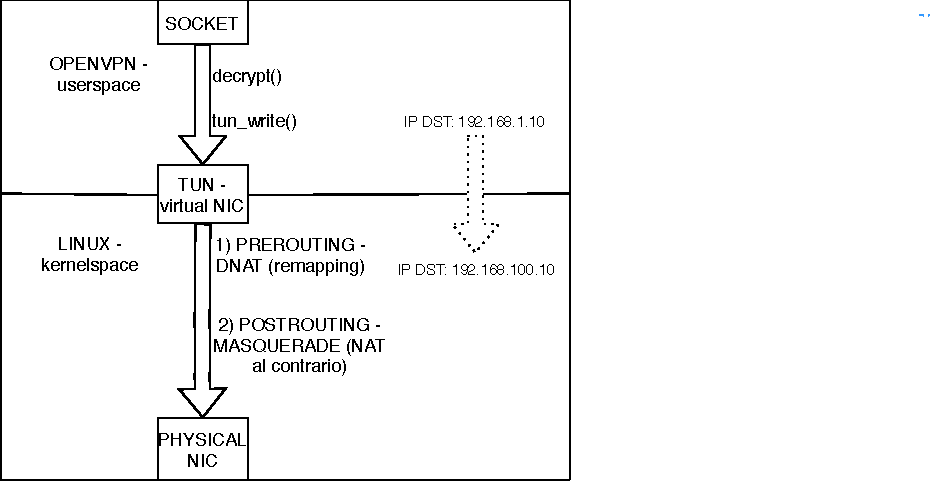
\includegraphics[scale=0.7]{img/ip_mapping_send}
  \label{fig:ip-mapping-send}
  \caption[IP Mapping: MoonCloud $\rightarrow$ Target]{
    IP Mapping: MoonCloud $\rightarrow$ Target. Si mostra un esempio di ciò che
    accade nel VPN client quando si riceve un pacchetto tramite la VPN.
    Per essere rigorosi occorre notare che una volta che OpenVPN invia qualcosa
    su un socker, il controllo passa di nuovo al sistema operativo che scrive
    quindi il pacchetto sulla scheda di rete fisica, ma questo non è di interesse
    per il problema in questione.}
\end{figure}

\begin{figure}
  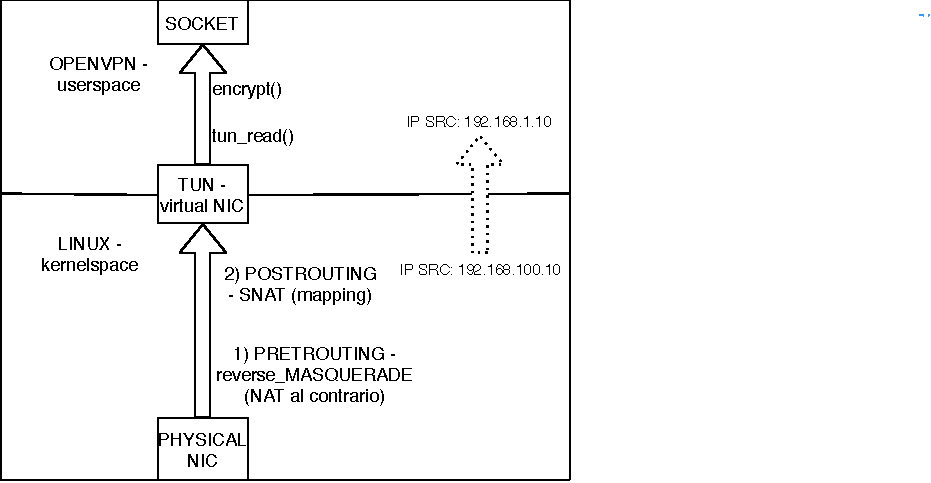
\includegraphics[scale=0.7]{img/ip_mapping_recv}
  \label{fig:ip-mapping-recv}
  \caption[IP Mapping: Target $\rightarrow$ MoonCloud]{
    IP Mapping: Target $\rightarrow$ MoonCloud. In questo caso si mostra
    cosa succede con i pacchetti in risposta a richieste provenienti
    da MoonCloud lungo la VPN.}
\end{figure}
